\begin{figure}[h!]
    \centering
    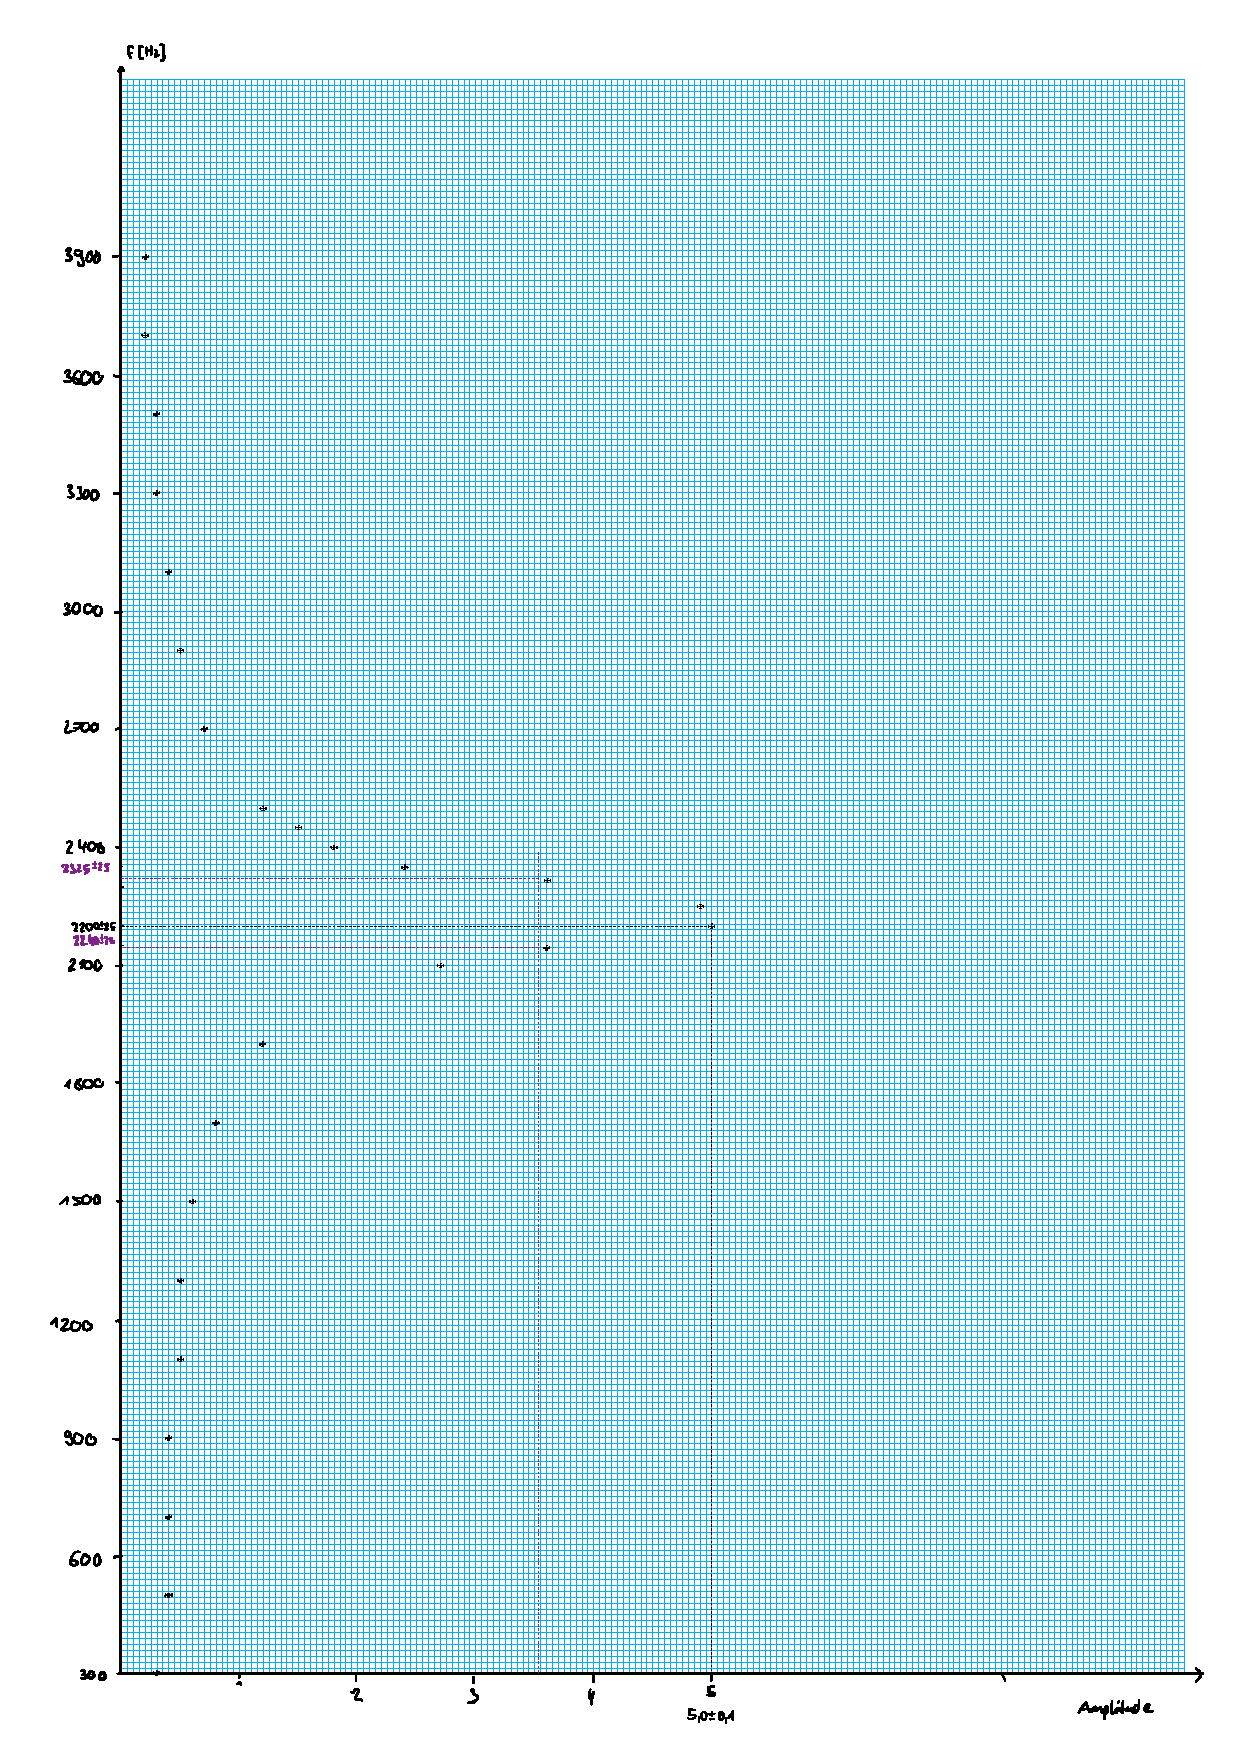
\includegraphics[page=1, width=.95\textwidth,]{Dias13.pdf}
    \caption{Diagramm 1: Amplituden Resonanz 1}
\end{figure}
\clearpage
\newpage
\begin{figure}[h!]
    \centering
    \includegraphics[page=2, width=1\textwidth,]{Dias13.pdf}
    \caption{Diagramm 2: Amplituden Resonanz 2}
\end{figure}
\newpage
\begin{figure}[h!]
    \centering
    \includegraphics[page=3, width=1\textwidth,]{Dias13.pdf}
    \caption{Diagramm 3: Amplituden Dämpfung 1}
\end{figure}
\newpage
\begin{figure}[h!]
    \centering
    \includegraphics[page=4, width=0.95\textwidth,]{Dias13.pdf}
    \caption{Diagramm 4: Amplituden Dämpfung 2}
\end{figure}
\newpage

\section{Aufgabe I}

\begin{table}[h!]
    \centering
    \begin{tabular}{c r r}
        \toprule
        Messung & Gemessene Zeit [s] & Umlaufzeit $T_0$ [s] \\
        \midrule
        1 & $36,32 \pm 0,3$ & $ 1,816 \pm 0,015$ \\
        2 & $36,34 \pm 0,3$ & $ 1,817 \pm 0,015$ \\
        3 & $36,31 \pm 0,3$ & $ 1,816 \pm 0,015$ \\
        \bottomrule
    \end{tabular}
\end{table}
Fehler:
\[\boxed{\overline{T_0} = 1,816 \pm 0,015}\]
\begin{equation}
    \Delta \overline{T_0} = \sqrt{\sigma^2 + (\Delta T_0)^2}
\end{equation}

Es ergibt sich ebenfalls für die Frequenz:

\[\boxed{f_0 = 0,551 \pm 0,005 \si{Hz}}\]

Wobei $\Delta T_0$ die Abweichung einer Umlaufzeit ist, also die Reaktionszeit heruntergerechnet auf einen Umlauf und $\sigma$ die
mittlere Abweichung des Mittelwerts ist.

%##############################################################

\section{Aufgabe II}
Hier wird für die Spannung $320$ mA der Index 1 und für die Spannung $400$ mA der Index 2 verwendet. 
Aus Diagramm 1 und 2 folgen für die Umlaufanzahlen bei halber Amplitude:

\[n_1 = 4,08 \pm 0,12\quad n_2 = 2,60 \pm 0,09\]

Die Umlaufzeiten betragen:

\[T_1 = 1,390 \pm 0,015\quad T_2 = 0,905 \pm 0,015\]

Damit ergeben sich nach Gleichung \ref{eq:delta} die Dämpfungskonstanten:

    \[\boxed{\delta_{a1} = \SI{0,122 \pm 0,004}{\tfrac{1}{\second}}}\notag\]
    \[\boxed{\delta_{a2} = \SI{0,295 \pm 0,011}{\tfrac{1}{\second}}}\notag\]

Fehler:

\[\Delta \delta=\ln(2) \sqrt{\frac{(T_{1/2})^{2} (\Delta n_{1/2})^{2} + (\Delta T_{1/2})^{2} (n_{1/2})^{2}}{(T_{1/2})^{4} (n_{1/2})^{4}}}\]

%##############################################################

\section{Aufgabe III}

Die Eigenfrequenz des Pendels $\omega_0$ berechnet sich nach Gleichung \ref{eq:eigen} mit den Messwerten des ungedämpften Pendels.
Dafür wird die Umlaufzeit aus Aufgabe I verwendet.
\[\omega_0 = 3,460 \pm 0,029 \si{Hz}\]
Dabei wurde für den Fehler folgende Formal verwendet:
\begin{equation}
   \Delta \omega_0 = \frac{2\pi}{T_0^2}\Delta T_0
\end{equation}

Nun ist anhand der Diagramme 3 und 4 zu bestimmen wo sich die jeweiligen Maxima der Amplituden befinden.
Daraus kann die Frequenz des Motors bei welcher die Amplitude  maximal wird bestimmt werden.
Im folgenden werden Index 1 zu Diagramm 3 und Index 2 zu Diagramm 4 zugeordnet.
Als gemessene Frequenz wird der Mittelwert der Frequenzen genommen:
\[ f_1 = 2200 \pm 25\ \si{Hz}\]
\[ f_2 = 2225 \pm 25\ \si{Hz} \]
\[\Rightarrow f = 2213 \pm 18 \ \si{Hz}\]

Der Fehler berechnet sich durch:
\begin{equation}
    \Delta f = \frac{\sqrt{2}}{2}\Delta f_{1/2}
\end{equation}

Daraus ergibt sich mit dem Faktor $\frac{1}{4000}$,da dies der Umrechnungsfaktor zwischen Funktionengenerator und Motor ist, die Frequenz des Motors und damit die des Pendels:

\[\boxed{f_{res} = 0,553 \pm 0,005 \si{Hz}}\]

\subsection{Bestimmung von $\delta$ durch die Halbwertsbreite}

Mit den Ergebnissen aus Diagramm 3 und 4 werden mithilfe von Gleichung \ref{eq:halb} die Dämpfungskonstanten bestimmt.
Dafür werden die Frequenzen gesucht, bei denen die Amplitude die hälfter der maximal Amplitude beträgt. Der Abstand ist dann die Halbwertsbreite $H$.
Jedoch muss die Frequenz $f$ erst in $\omega = \frac{2 \pi}{4000} f$ umgerechnet werden.

\[\boxed{\delta_{b1}= \SI{0,067 \pm 0,028}{\tfrac{1}{\second}}}\]
\[\boxed{\delta_{b2} = \SI{0,255 \pm 0,028}{\tfrac{1}{\second}}}\]

Der Fehler wird wie folgt berechnet:

\begin{equation}
    \Delta \delta = \frac{2 \cdot \pi}{2 \cdot 4000}\sqrt{(\Delta\omega_2)^2+ (\Delta\omega_1)^2}
\end{equation}
\newpage

\subsection{Bestimmung von $\delta$ durch Resonanzüberhöhung}

Für die Bestimmung der Dämpfungskonstanten mithilfe der Resonanzüberhöhung werden die Maximalamplituden aus den Diagrammen 3 und 4 errmittelt.
Als den Wert für $b(\omega \rightarrow 0)$ wird hier jeweils der kleinste messbare Wert verwendet und für die Maximalamplituden $b(\omega')$ der jeweils abgelesene Wert.
Aus diesen Werten können mit Gleichung \ref{eq:deltafertig} die Dämfungskonstanten bestimmt werden:

\[\boxed{\delta_{c1} = \SI{0,10 \pm 0,03}{\tfrac{1}{\second}}}\]
\[\boxed{\delta_{c2} = \SI{0,22 \pm 0,05}{\tfrac{1}{\second}}}\]

Dabei wurde der Fehler wie folgt berechnet:

\begin{equation}
    \Delta \delta = \sqrt{
\left( \frac{b(\omega \to 0)}{2 b(\omega')} \cdot \Delta \omega_0 \right)^2
+ \left( \frac{\omega_0}{2 b(\omega')} \cdot \Delta b(\omega \to 0) \right)^2
+ \left( - \frac{\omega_0 b(\omega \to 0)}{2 b(\omega')^2} \cdot \Delta b(\omega') \right)^2
}
\end{equation}
